% Appendix A

\chapter{\textit{Datasheet} LaRE - Protótipo} 
\label{AppendixA}

\begingroup
\setlength{\columnsep}{10pt} % Ajusta o espaçamento entre colunas, se necessário

% LOGO
\begin{figure}[hbtp] % [H] fixa a posição
    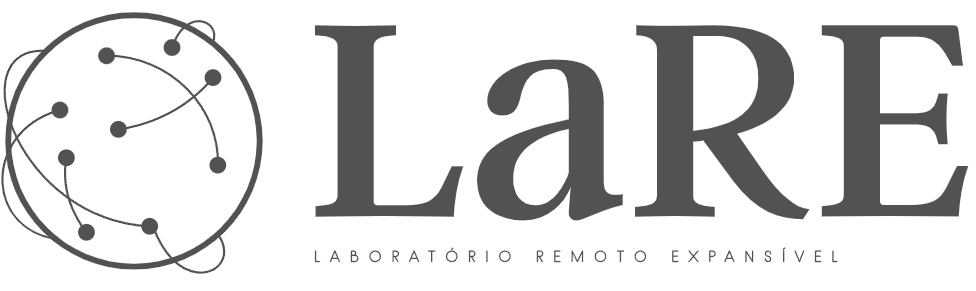
\includegraphics[width=0.4\textwidth]{figures/logo.jpg}
\end{figure}

% CARACTERÍSTICAS E IMAGEM LORE
\begin{figure}[hbtp]
\begin{minipage}{0.47\textwidth}

\section{Características}
\begin{itemize}
    \item Matriz com 3 placas baseadas nas dimensões PC/104;
    \item Fonte de alimentação-\SI{5}{\volt}/\SI{1}{\ampere},\newline baseado no LM317\footnote{\href{https://www.ti.com/lit/ds/symlink/lm317.pdf}{Datasheet LM317}};
    \item Experiências:
    \begin{itemize}
        \item Lei de Ohm;
        \item Retificador de meia onda e onda completa;
        \item Filtros passa-alto e passa-baixo.
    \end{itemize}
\end{itemize}

\end{minipage}
\hfill
\begin{minipage}{0.47\textwidth}
    \centering
    \includegraphics[width=0.45\textwidth]{figures/lore.jpg}
\end{minipage}
\end{figure}

\newpage

\section{Descrição}
A matriz de relés do LaRE é constituida por três placas: placa de alimentação, placa com o circuito da Lei de Ohm e a placa com os circuitos dos filtros e rectificadores. A matriz do LaRE é controlada pelo RaspberryPI. Há vários tipos de alimentação: \SI{220}{\volt} AC que alimenta o rectificador de onda completa; o VirtualBench fornece alimentação de \SI{12}{\volt} DC ao LM317 e aos registos de deslocamento, sn74hc595\footnote{\href{https://www.ti.com/lit/ds/symlink/sn74hc595.pdf}{Datasheet SN74HC595}} e fornece tensão variável 0-\SI{5}{\volt} DC ao circuito da Lei de Ohm. Os ULN2003a\footnote{\href{https://www.ti.com/lit/ds/symlink/uln2003a.pdf}{Datasheet ULN2003a}}, são alimentados pela fonte de alimentação, baseada no LM317, \SI{5}{\volt}.
Todas as medições são feitas pelo VirtualBench. 
\endgroup

\section{Aplicações}
\begin{itemize}
    \item Laboratórios Remotos;
    \item Experiências remotas;
    \item Estudo da Lei de Ohm;;
    \item Estudo de rectificadores;
    \item Estudo de filtros.
\end{itemize}
\newpage
\section{Especificações técnicas}
\begin{table}[htb]
\caption{Especificações técnicas genéricas - \textbf{Sujeito a mudança}}
\centering
\begin{tabular}{lcr}
\toprule
 & Unidades & Valores \\
\midrule
$I_{Max}$ do VirtualBench & $A$ & 0.5 \\
$I_{Max}$ da fonte \SI{5}{V} DC & $A$ & 1.5 \\
Transformador & $?$ & REVER \\
Dimensões placas & $mm*mm$ & 96x90 \\
\bottomrule
\end{tabular}
\end{table}

\begin{table}[htb]
\caption{Especificações técnicas genéricas dos relés - \textbf{Sujeito a mudança}}
\centering
\begin{tabular}{lcclllll}
\toprule
Relés & \multicolumn{2}{c}{Bobine} & \multicolumn{5}{c}{Contactos}\\
\midrule
& \multicolumn{1}{l}{$V_{Nominal}$} & \multicolumn{1}{l}{$V_{Max}$} & $P_{Max}$ & $V_{Max}$ & $I_{Max}$ & $I_{Max}$\\
\midrule
3570-1331-123  & \multirow{2}{*}{\SI{12}{\volt}} & \multirow{2}{*}{\SI{16}{\volt}}  & \multirow{2}{*}{\SI{10}{\watt}} & \multirow{2}{*}{$\SI{150}{\volt}_{DC}$} & \multirow{2}{*}{\SI{0.5}{\ampere}} & \multirow{2}{*}{\SI{1}{\ampere}}\\
3572-1220-123 & & & & & & &\\                
\bottomrule
\end{tabular}%
\end{table}

\begin{table}[htb]
\caption{Ligações entre placas - \textbf{Sujeito a mudança}}
\centering
\begin{tabular}{lr}
\toprule
\multicolumn{2}{c}{Tipo de ligações}\\
\midrule
RaspberryPI-LaRE & Conector IDC, fêmea, 40 pinos, \SI{2.54}{\mm}\\
Placa Lei de Ohm-Rectificadores/Filtros & Conector de 6 pinos Arduino Stackable\\
Placa Fontes de tensão-Rectificadores/Filtros &  Conector KK, \SI{2.54}{\mm}, M/F \\
\bottomrule
\end{tabular}
\end{table}
\raggedright

%%%%%%%%%%%%%%%%

\newpage

\section{Pinout}
\begin{figure}[hbtp]
    \centering
    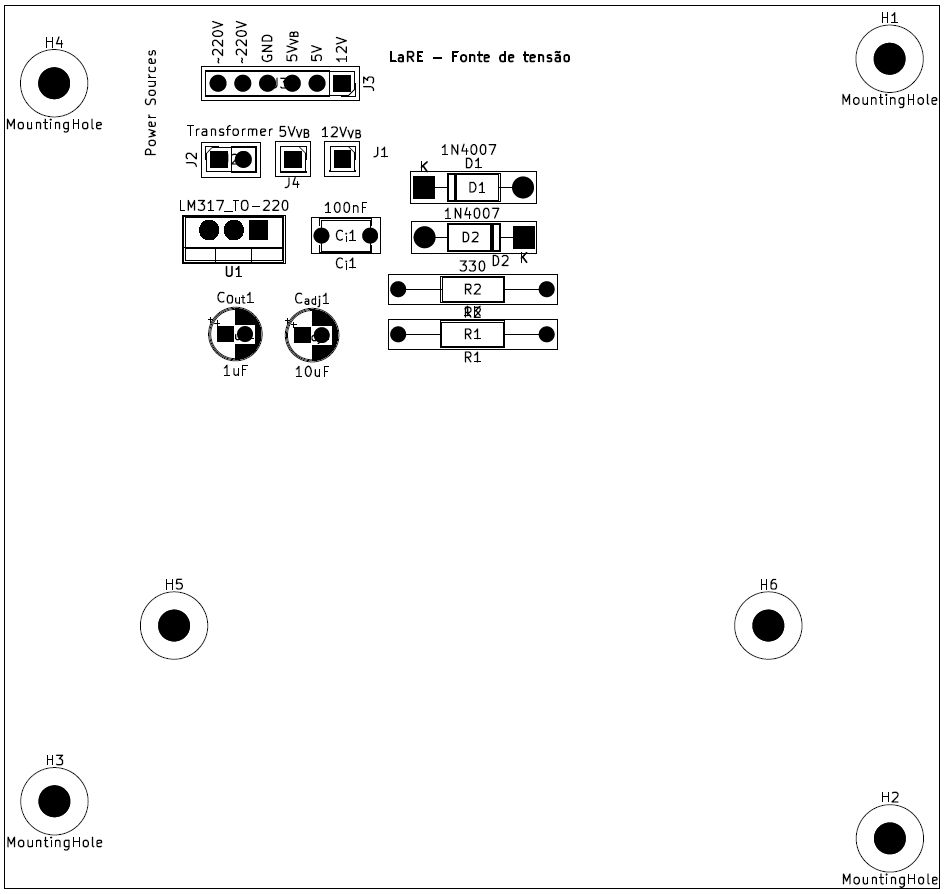
\includegraphics[width=1\textwidth]{figures/fonte_DATASHEET.png}
    \caption{LaRE - Pinout [Fonte de tensão]}
    \label{fig:arquitecturalore}
\end{figure}
\centering

\begin{figure}[hbtp]
    \centering
    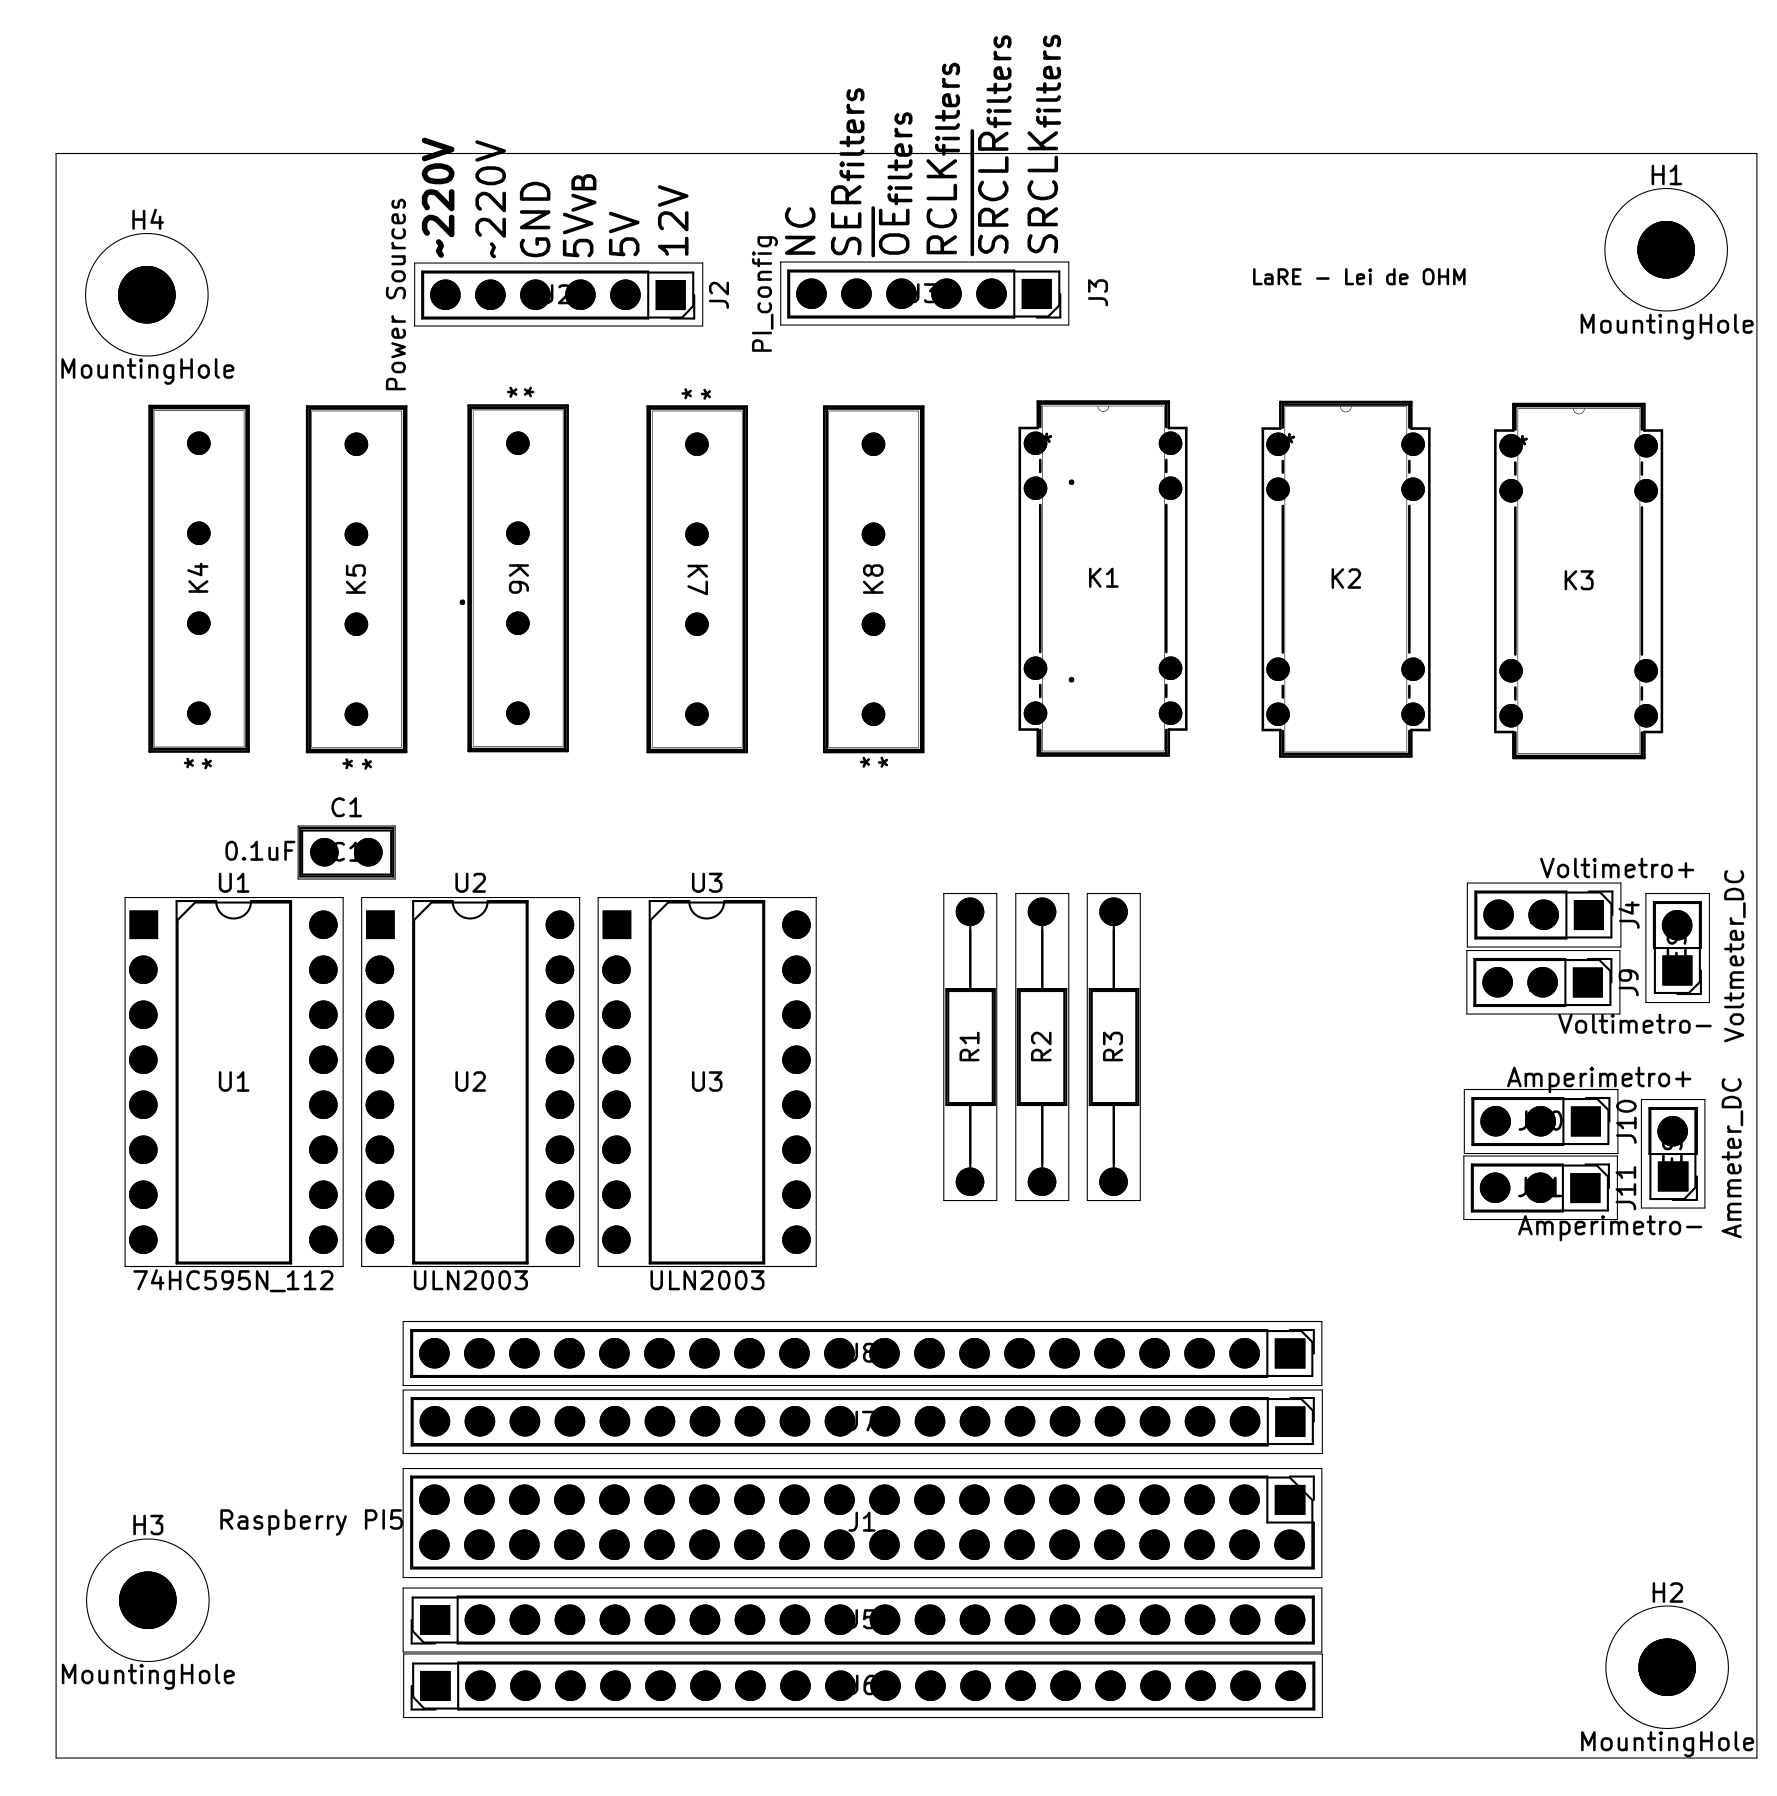
\includegraphics[width=1\textwidth]{figures/lei_ohm_PB.png}
    \caption{LaRE - Pinout [Lei de Ohm]}
    \label{fig:placaleiohm}
    \textbf{Os símbolos ** indicam o pino 1 dos relés}
\end{figure}
\centering

\begin{figure}[hbtp]
    \centering
    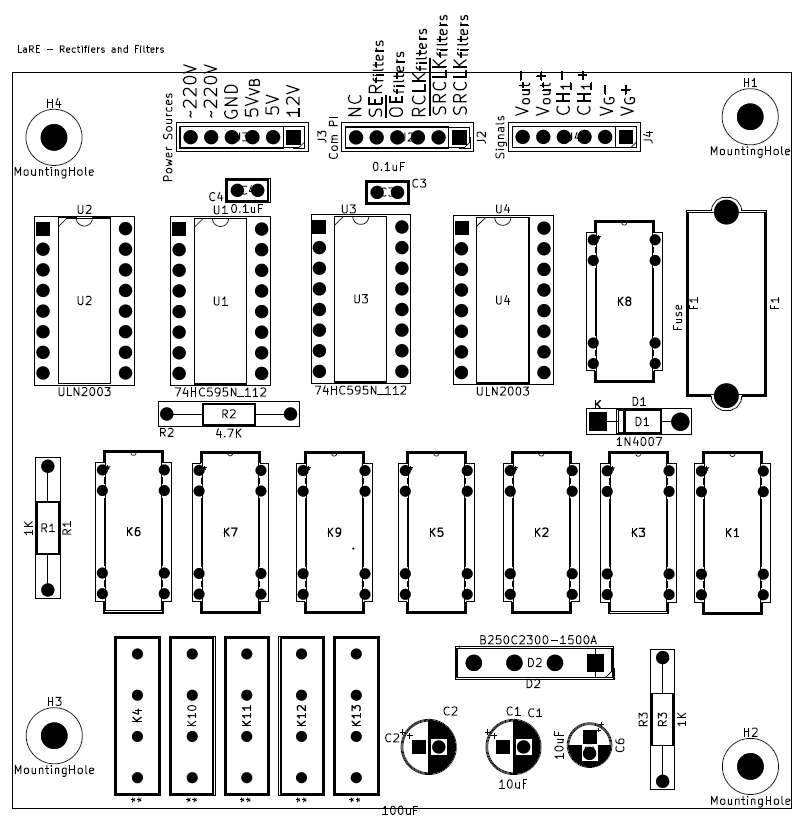
\includegraphics[width=1\textwidth]{figures/rectificador_DATASHEET.png}
    \caption{LaRE - Pinout [Rectificadores/Filtros]}
    \label{fig:rectificadoresfiltros}
\end{figure}
\centering

\newpage

\raggedright
\section{Dimensões mecânicas}
\begin{figure}[hbtp]
    \centering
    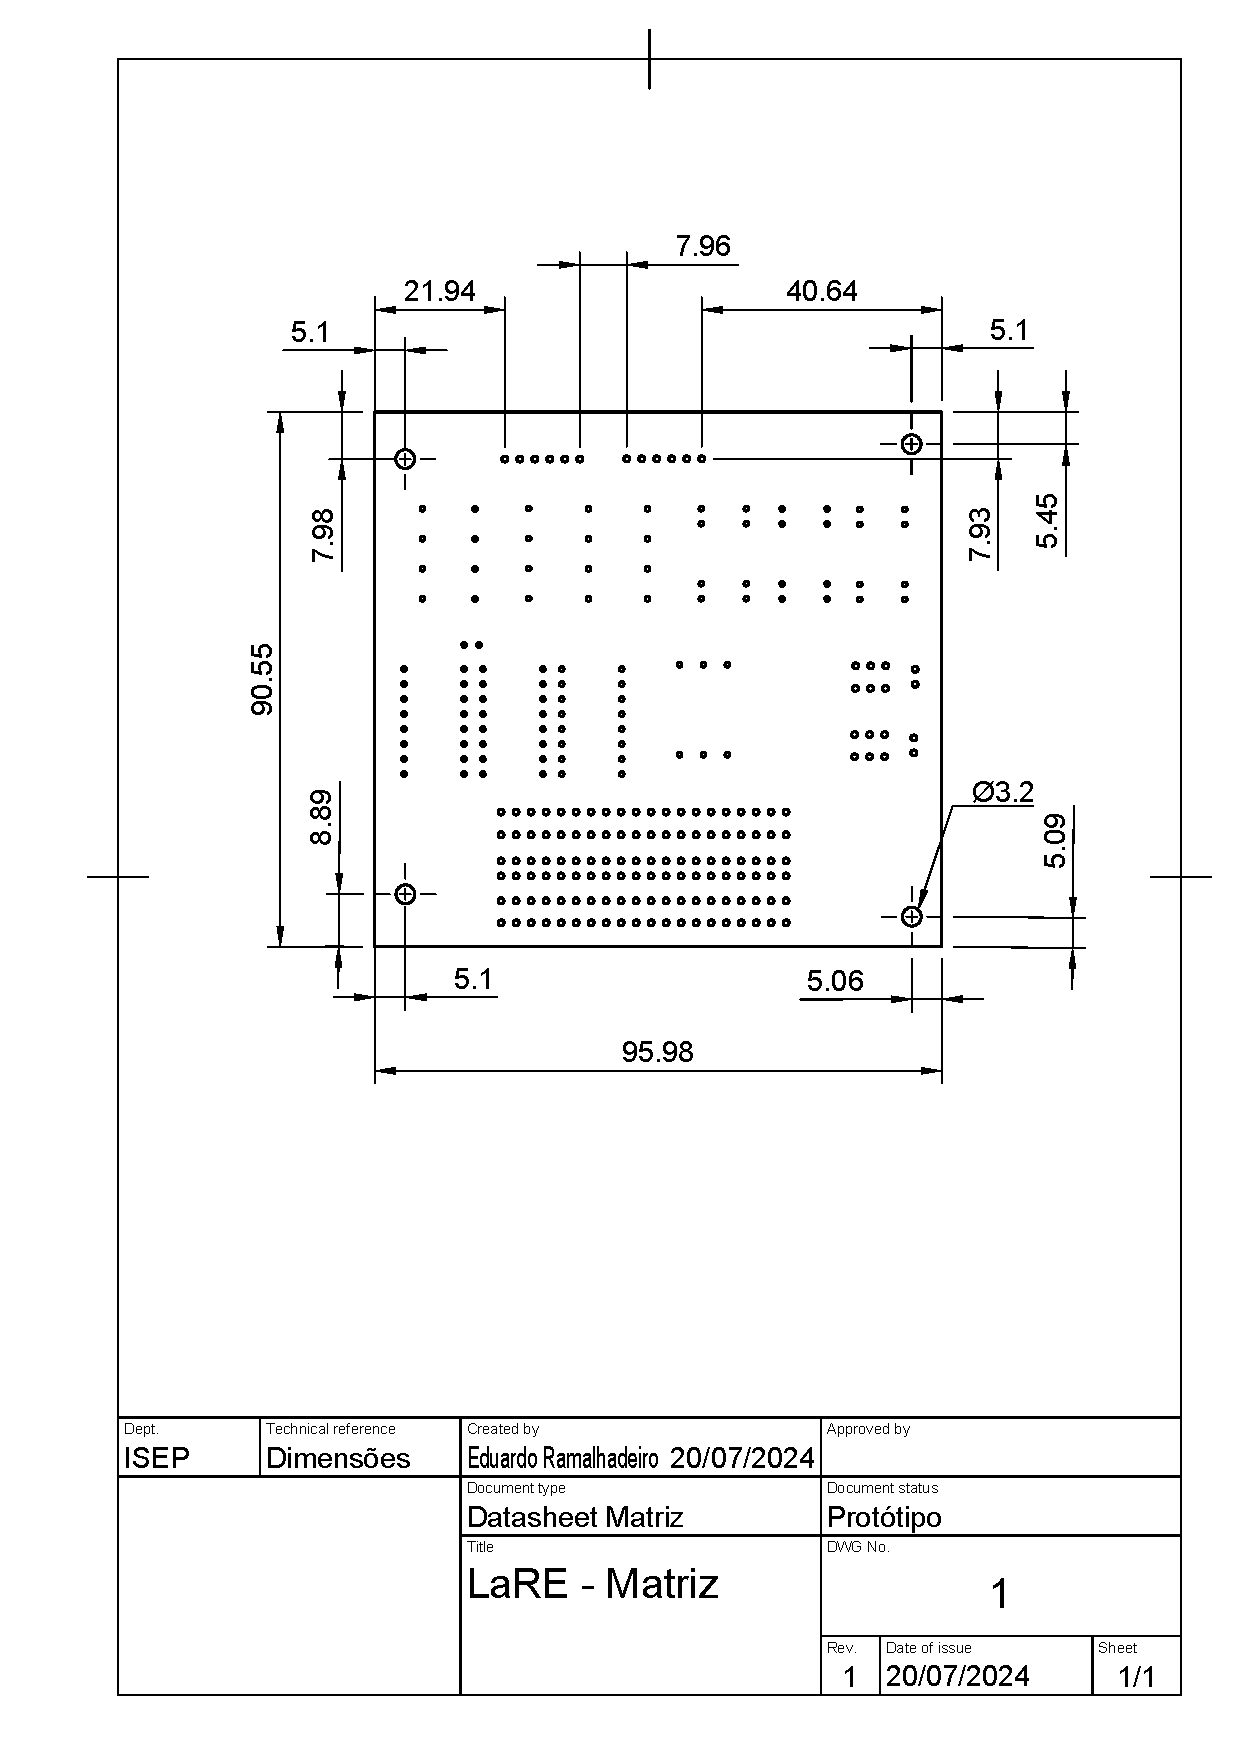
\includegraphics[width=0.8\textwidth]{figures/LaRE-dimesoes_mecanicas.pdf}
    \caption{Dimensões mecânicas PC/104 - LaRE}
    \label{fig:DimensõesmecânicasPC104}
\end{figure}

\raggedright
\begin{figure}[hbtp]
    \centering
    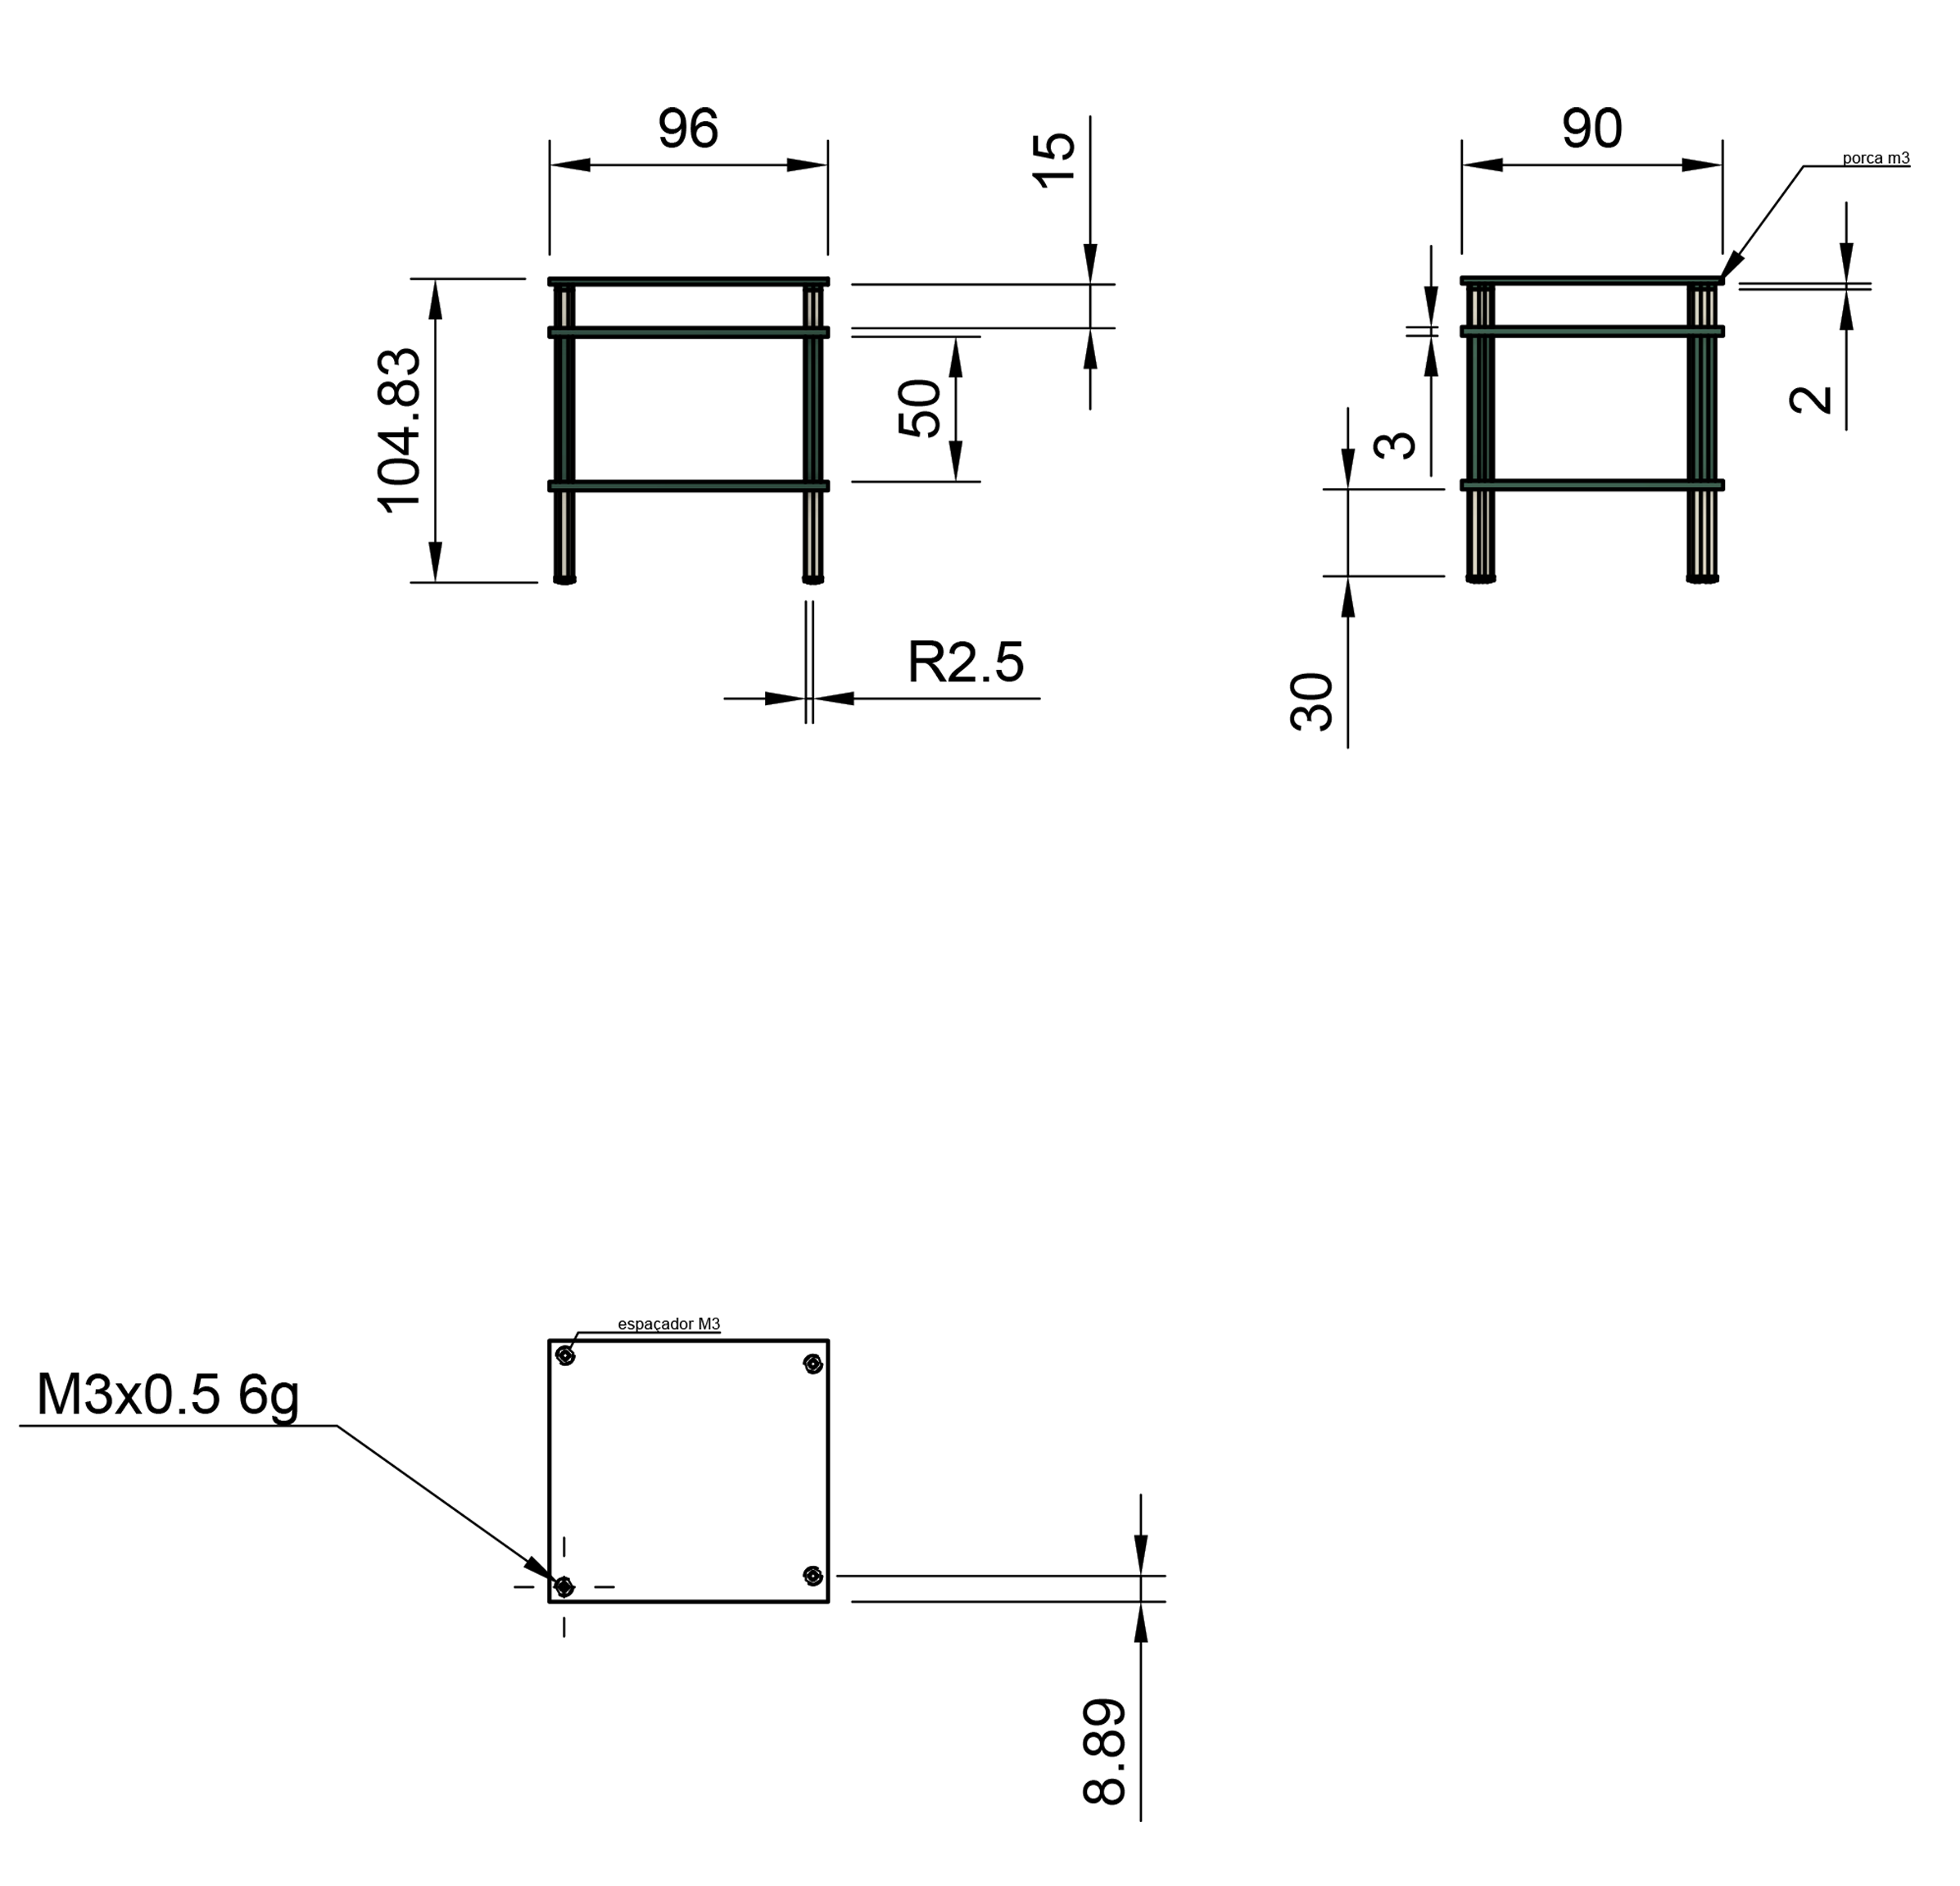
\includegraphics[width=1\textwidth]{figures/LaRE_desenhotecnico.png}
    \caption{Dimensões mecânicas LaRE}
    \label{fig:DimensõesmecânicasLaRE}
\end{figure}

\raggedright
\begin{figure}[hbtp]
    \centering
    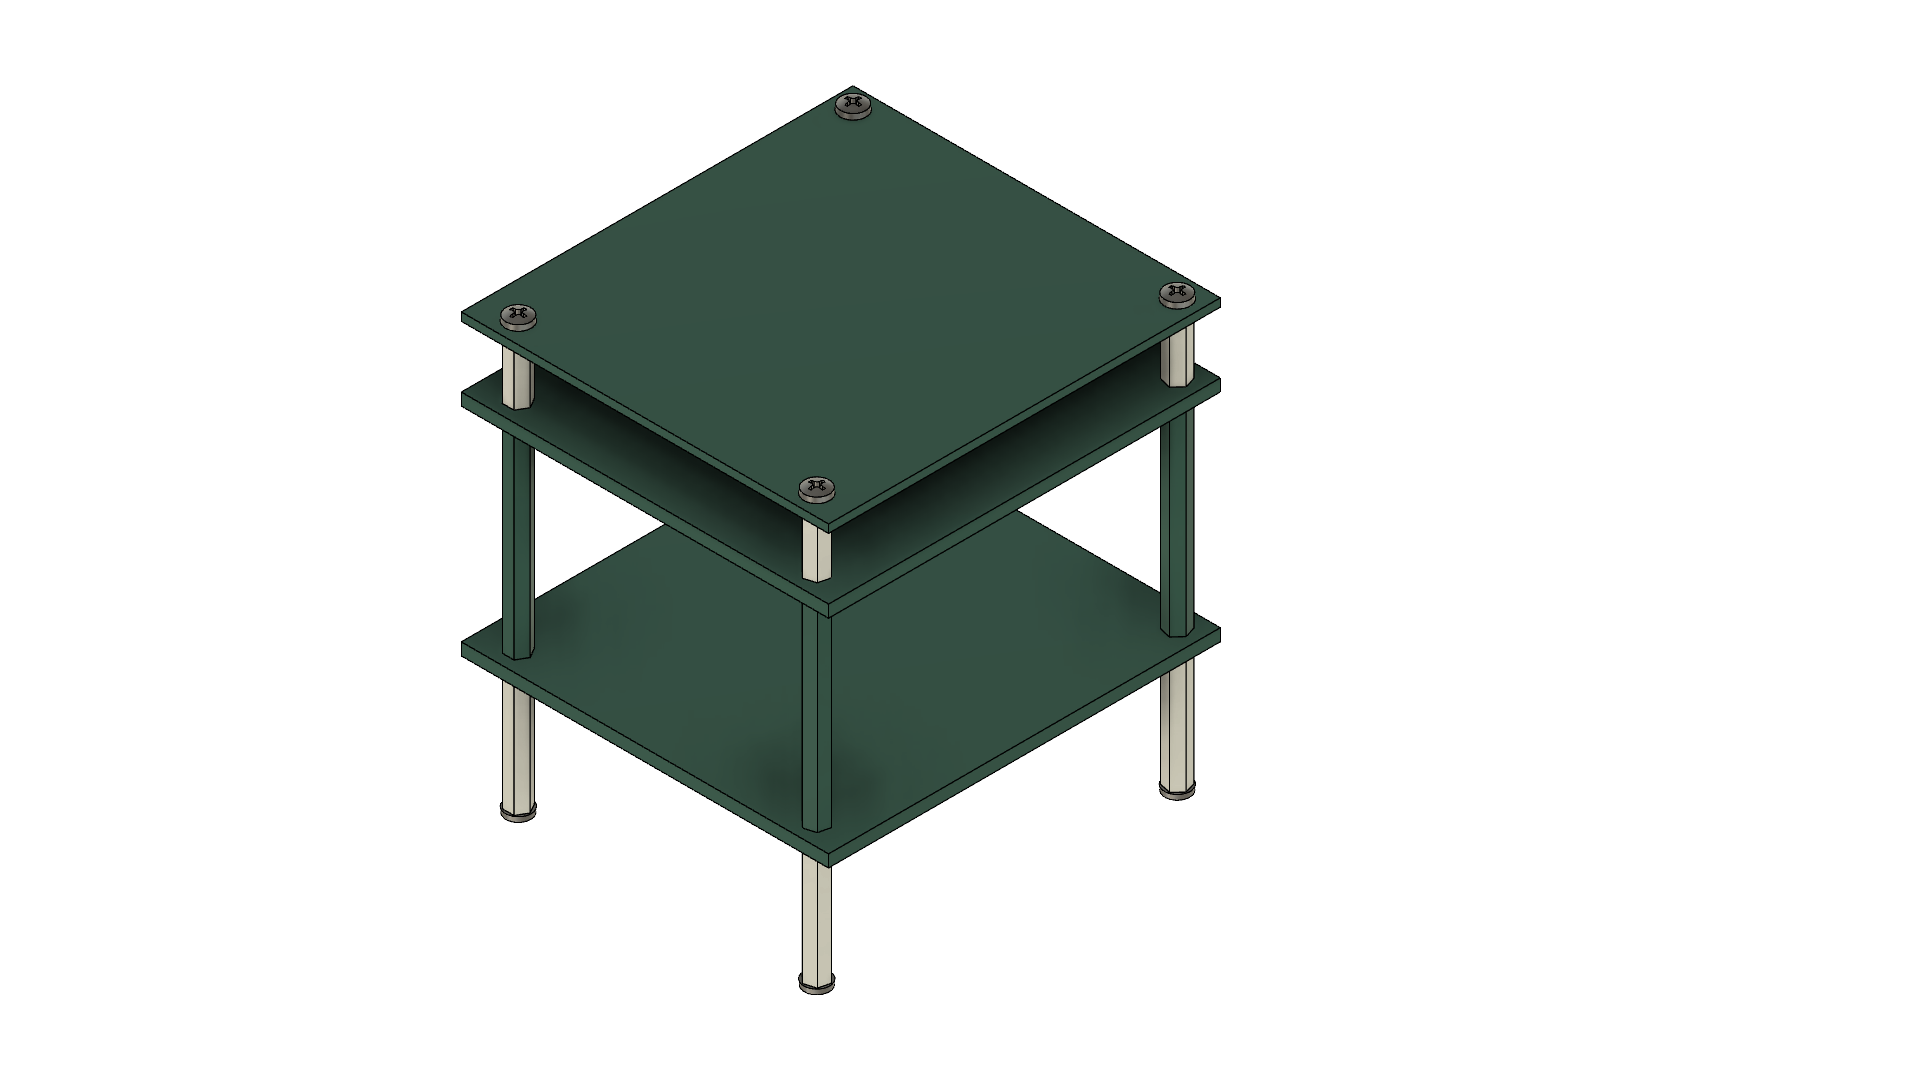
\includegraphics[width=1\textwidth]{figures/LaRE_esqueleto v2.png}
    \caption{Perspectiva LaRE}
    \label{fig:esqueletoLaRE}
\end{figure}

\newpage

\section{Esquemas elétricos}
\begin{figure}[hbtp]
    \centering
    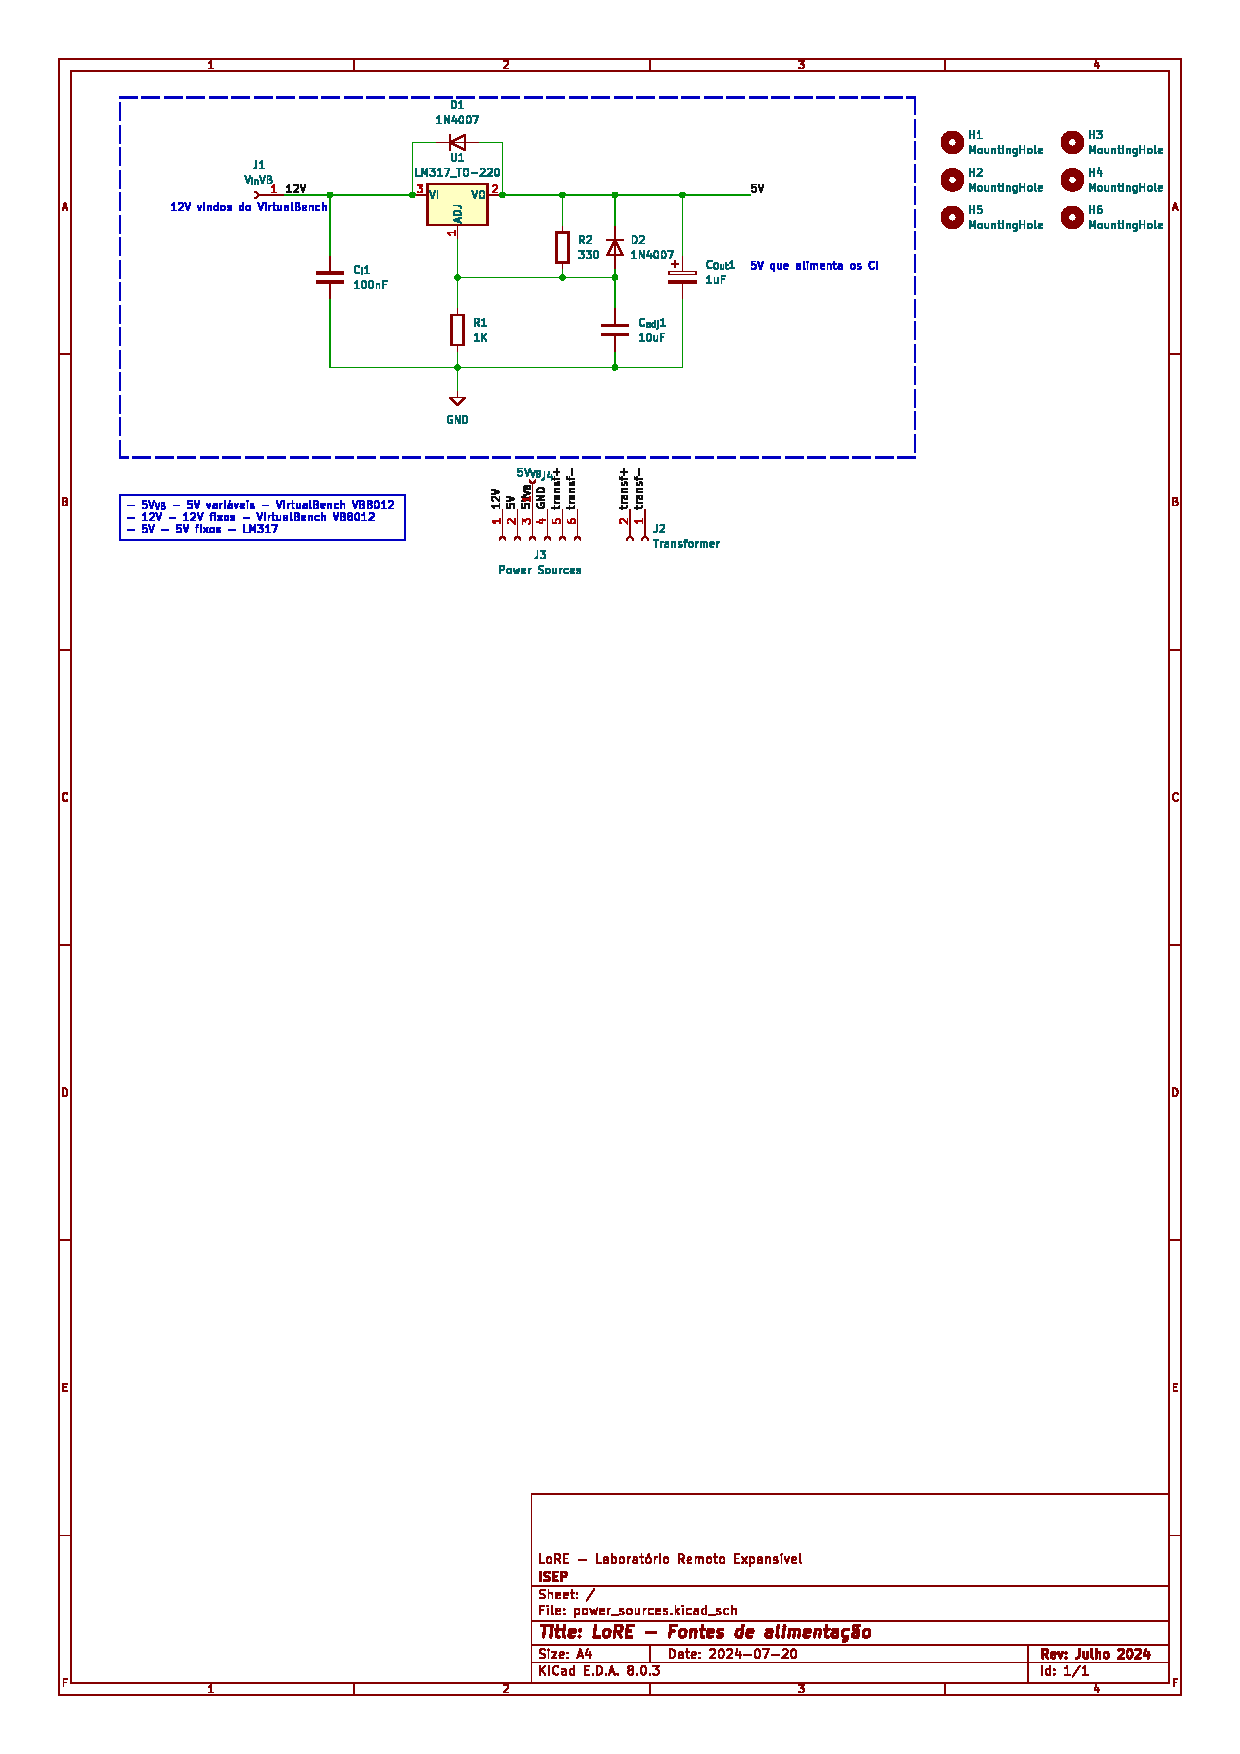
\includegraphics[width=0.8\textwidth]{figures/fonte_sch.pdf}
    \caption{LaRE - Esquema [Fonte de tensão]}
    \label{fig:esquemafonte}
\end{figure}
\centering

\begin{figure}[hbtp]
    \centering
    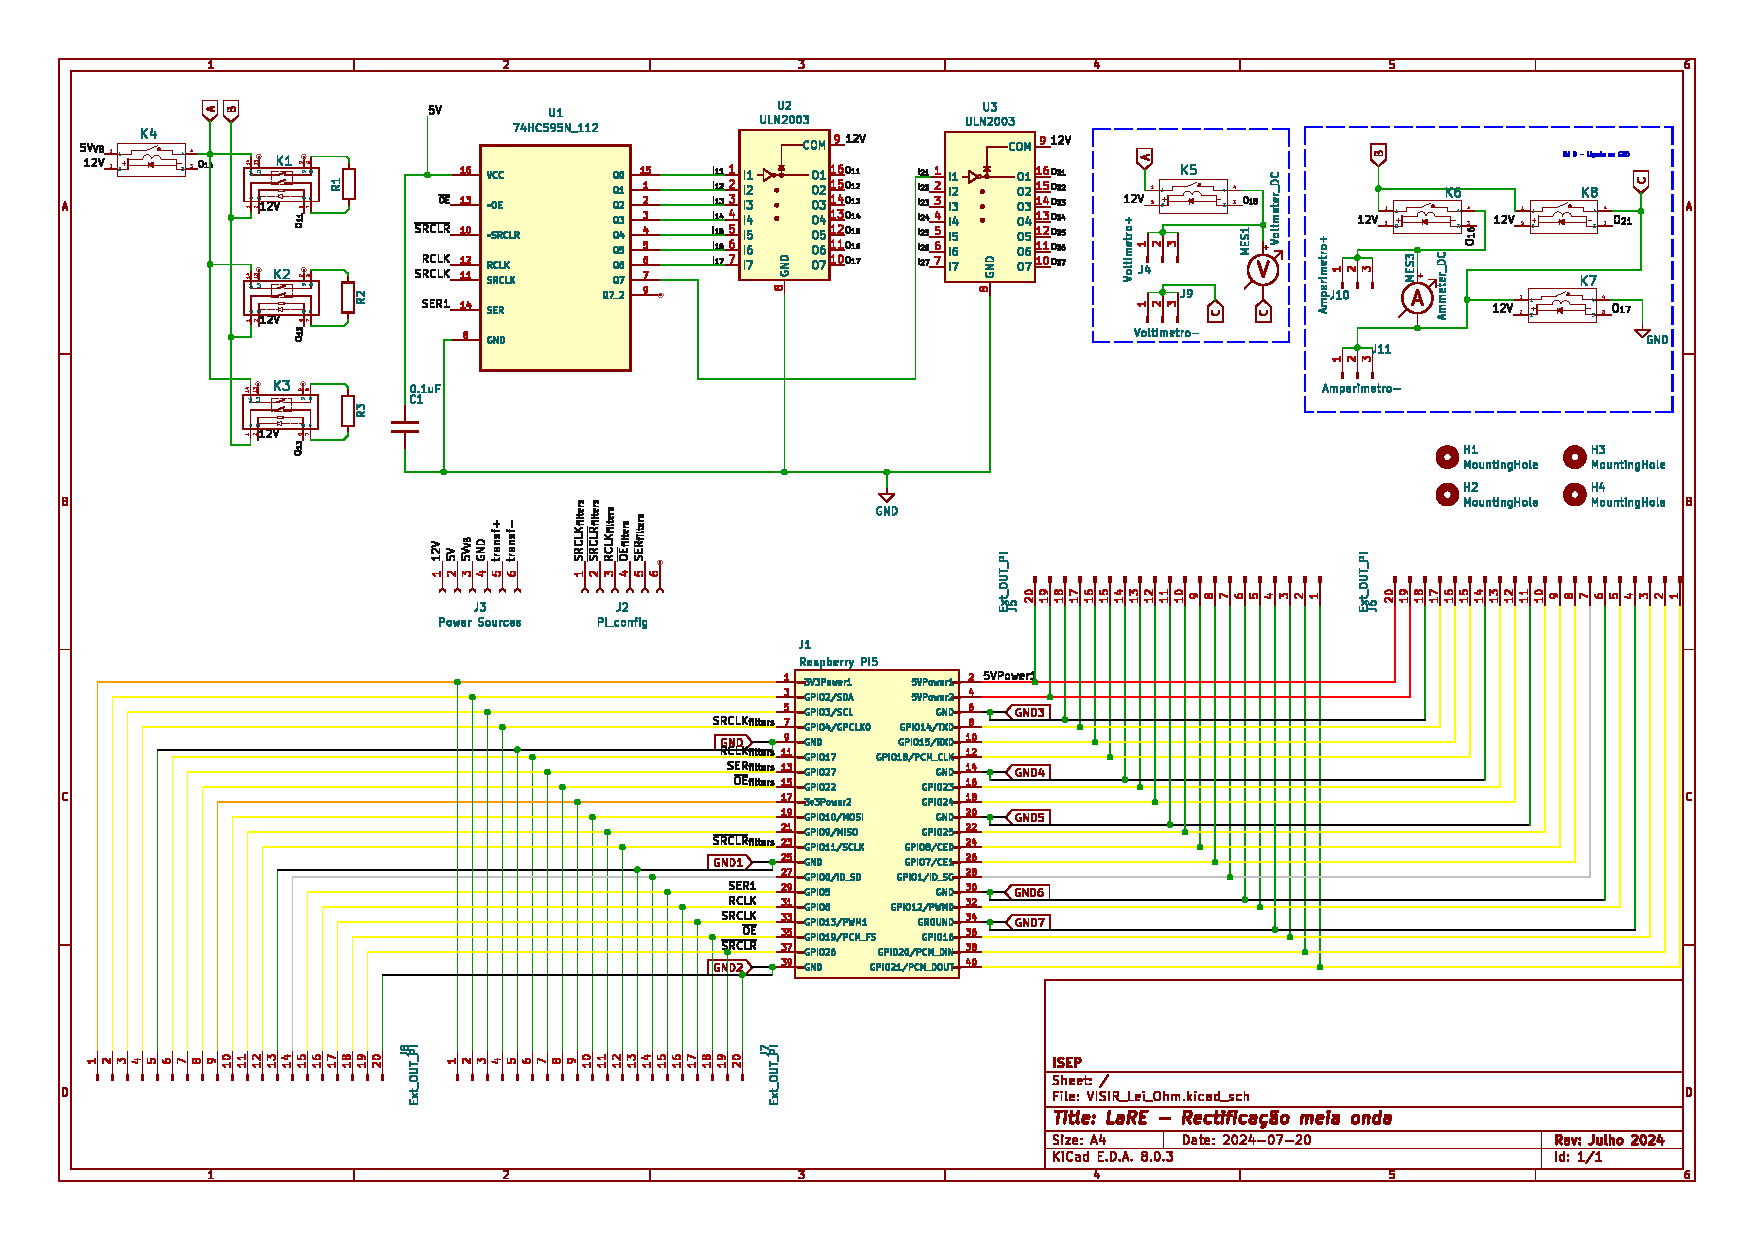
\includegraphics[width=1.4\textwidth, angle=-90]{figures/ohm_sch.pdf}
    \caption{LaRE - Esquema [Lei de Ohm]}
    \label{fig:esquemaohm}
\end{figure}
\centering


\begin{figure}[hbtp]
    \centering
    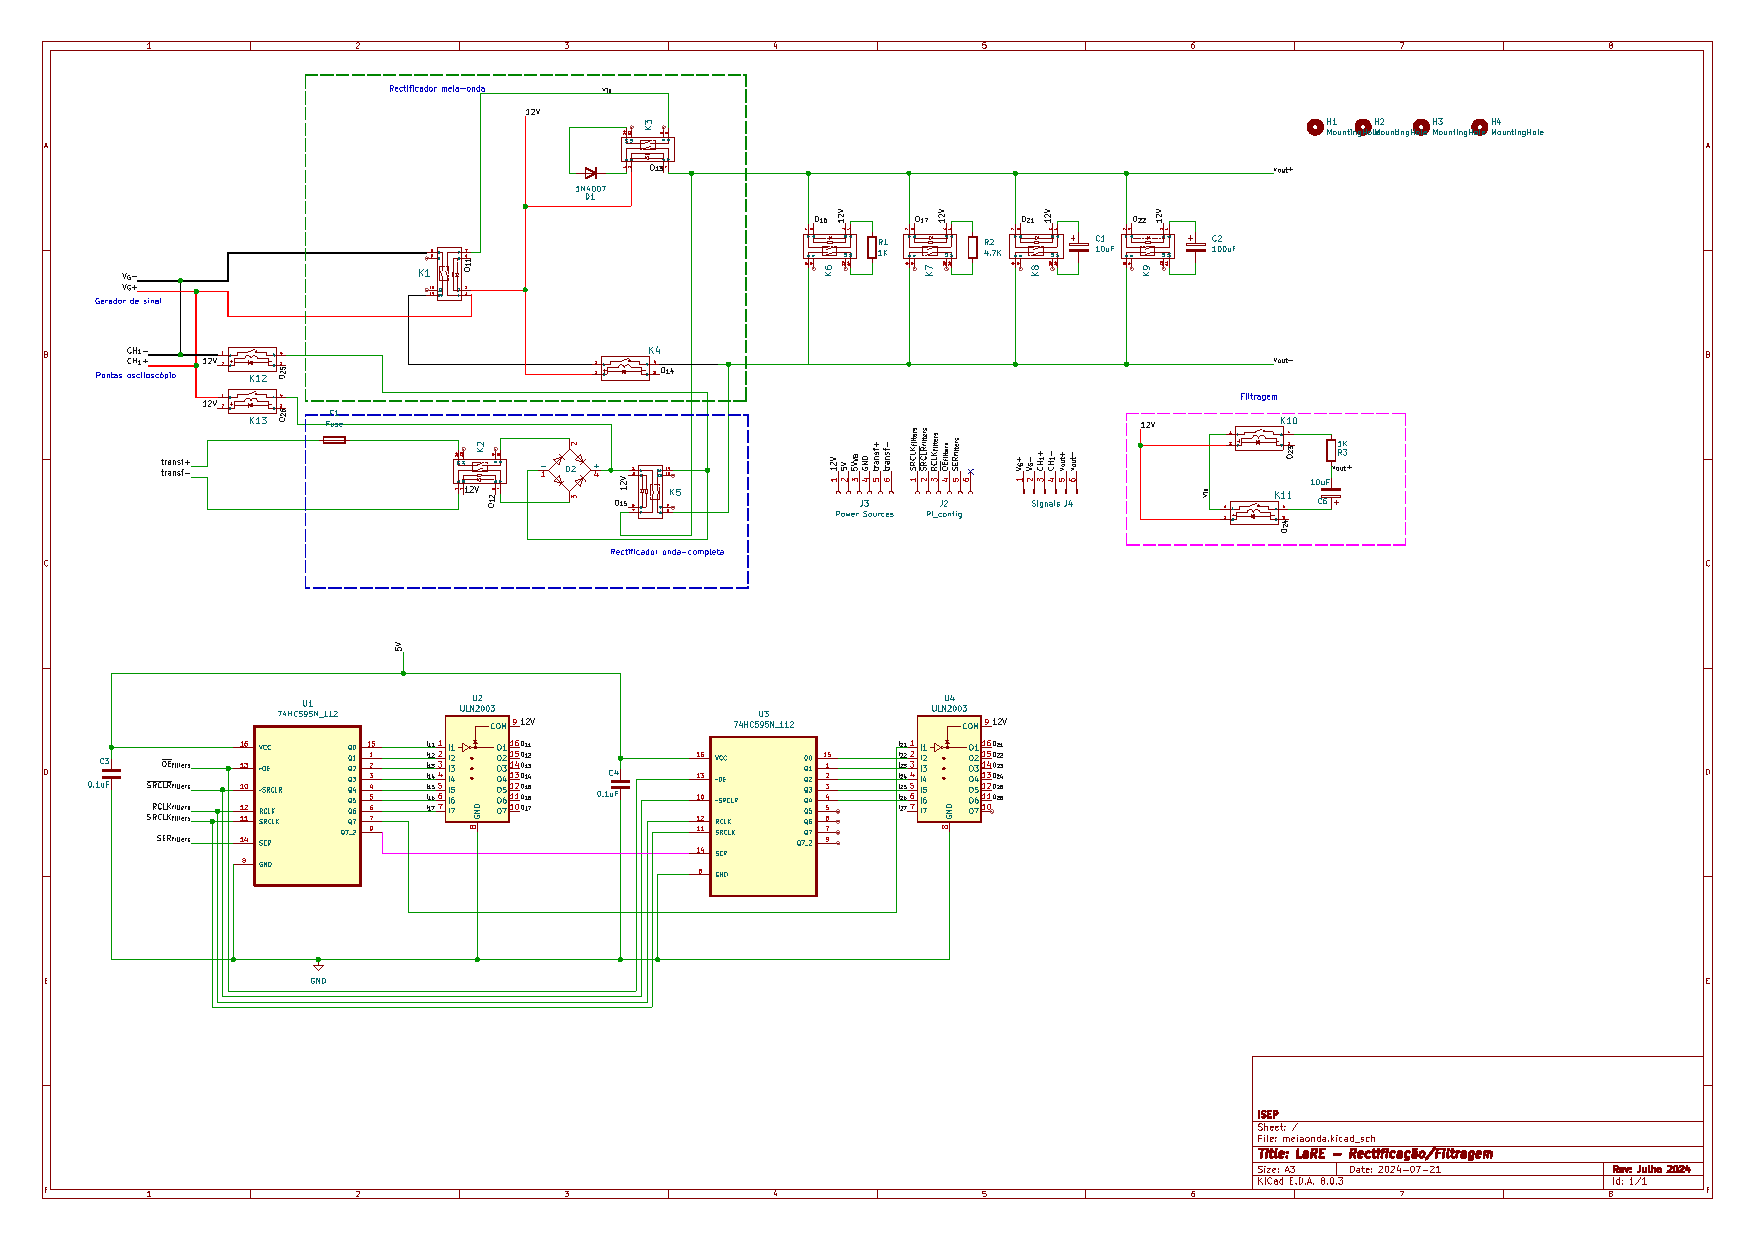
\includegraphics[width=1.4\textwidth, angle=-90]{figures/rectificacao_sch.pdf}
    \caption{LaRE - Esquema [Recficadores/Filtros]}
    \label{fig:esquemarectificador}
\end{figure}
\centering

\newpage

\section{Esquemas PCB}\begin{figure}[hbtp]
    \centering
    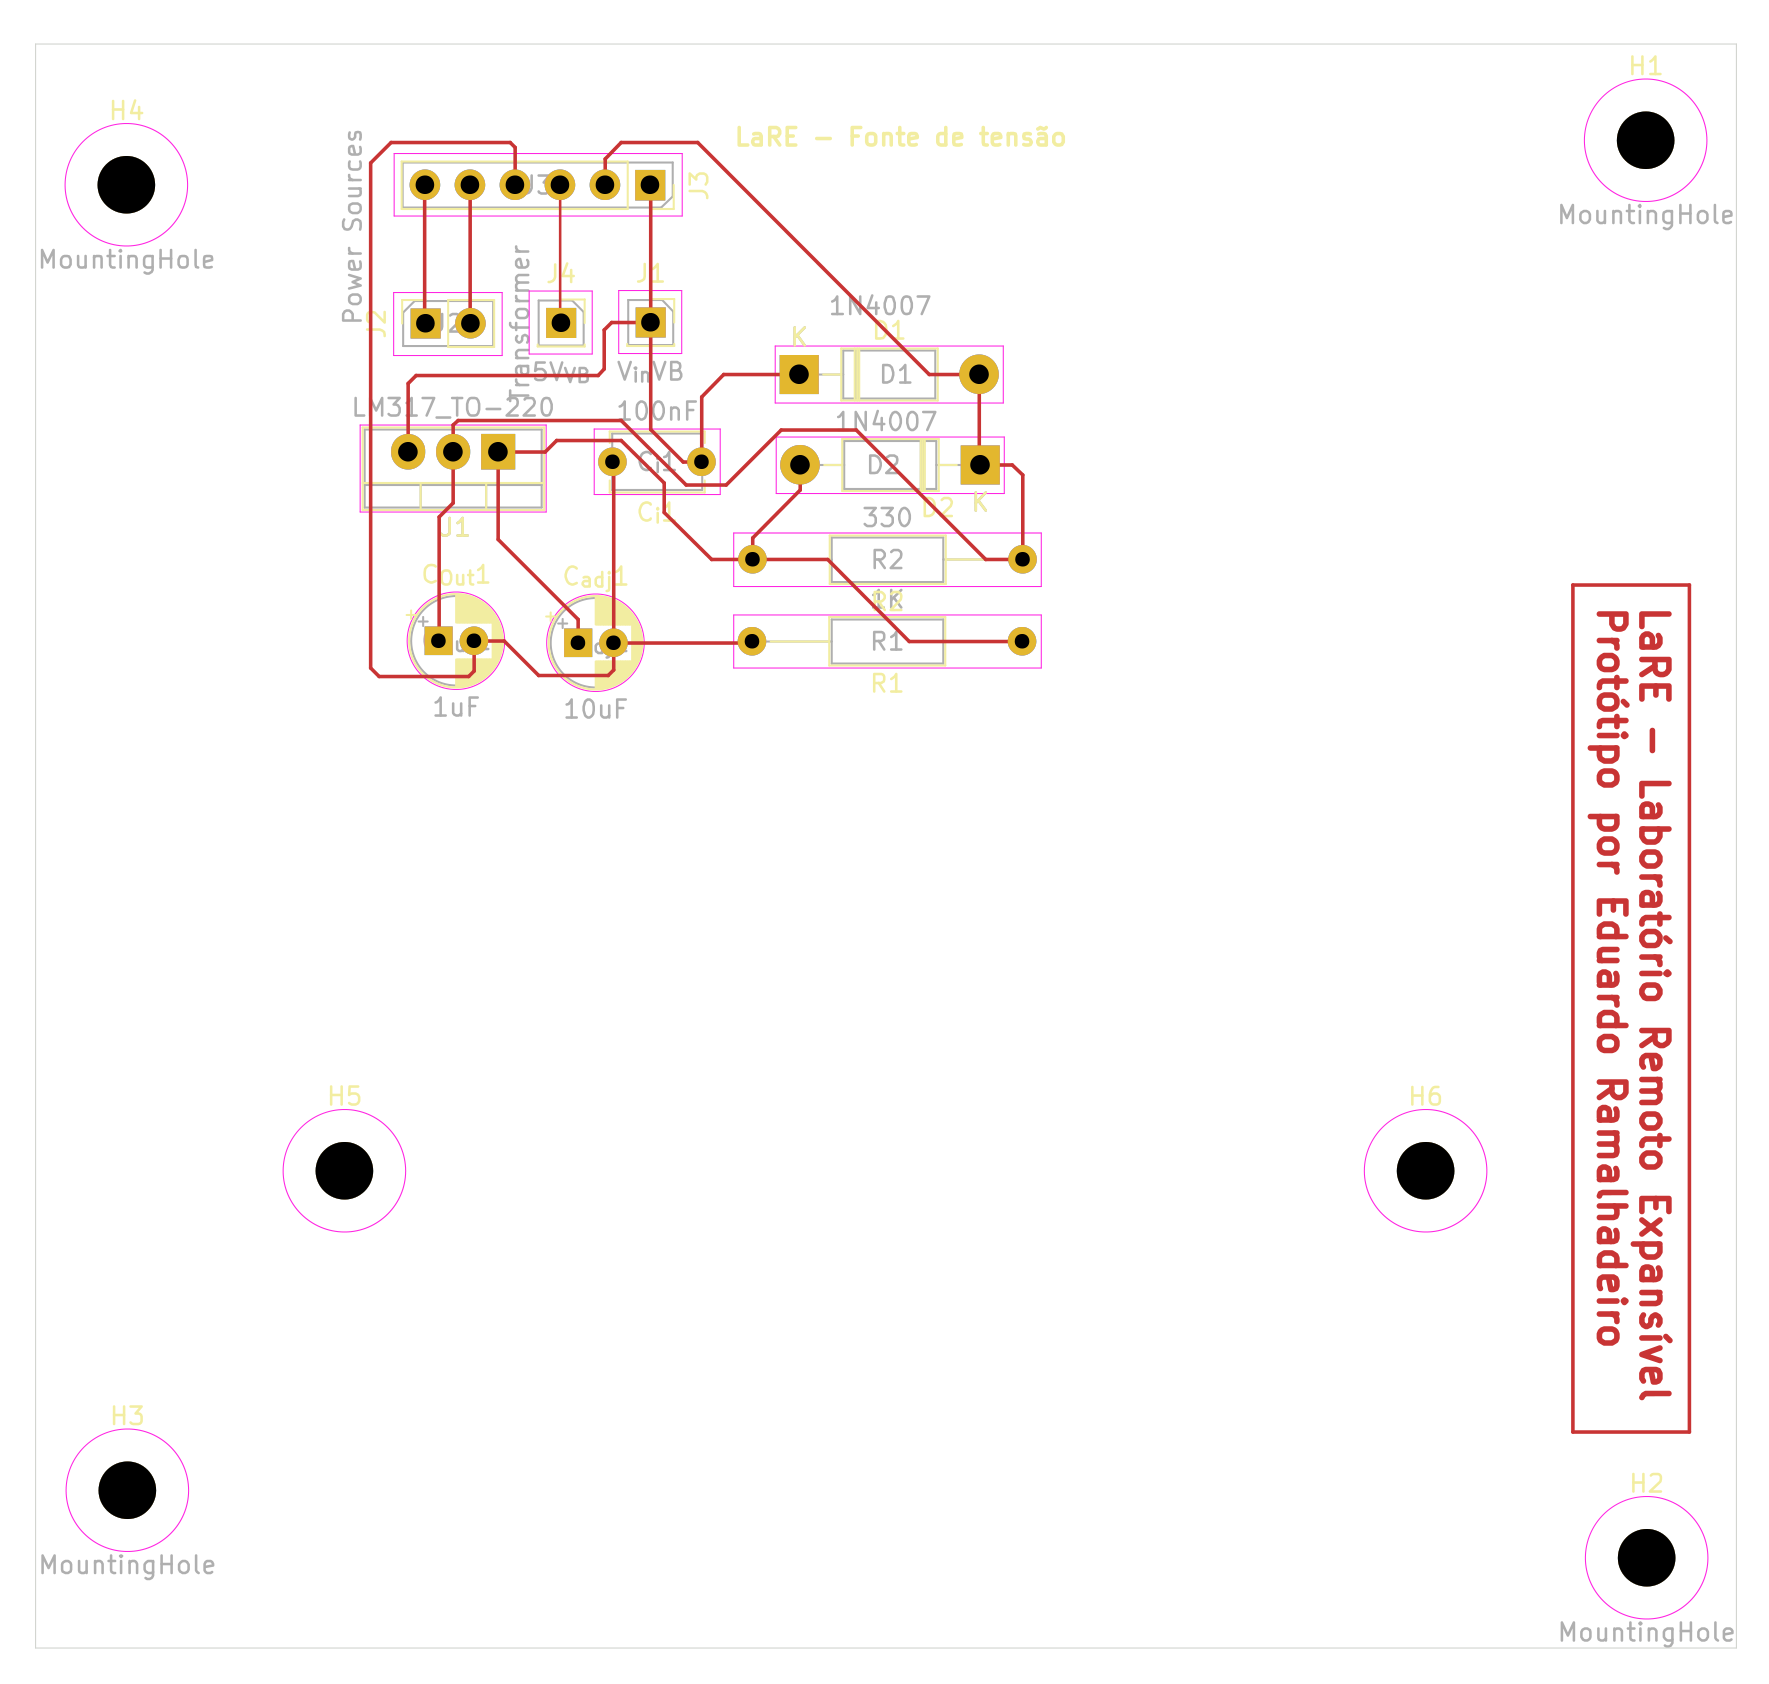
\includegraphics[width=1\textwidth]{figures/pcb_fonte.png}
    \caption{LaRE - PCB [Fonte de tensão]}
    \label{fig:pcbfonte}
\end{figure}
\centering

\begin{figure}[hbtp]
    \centering
    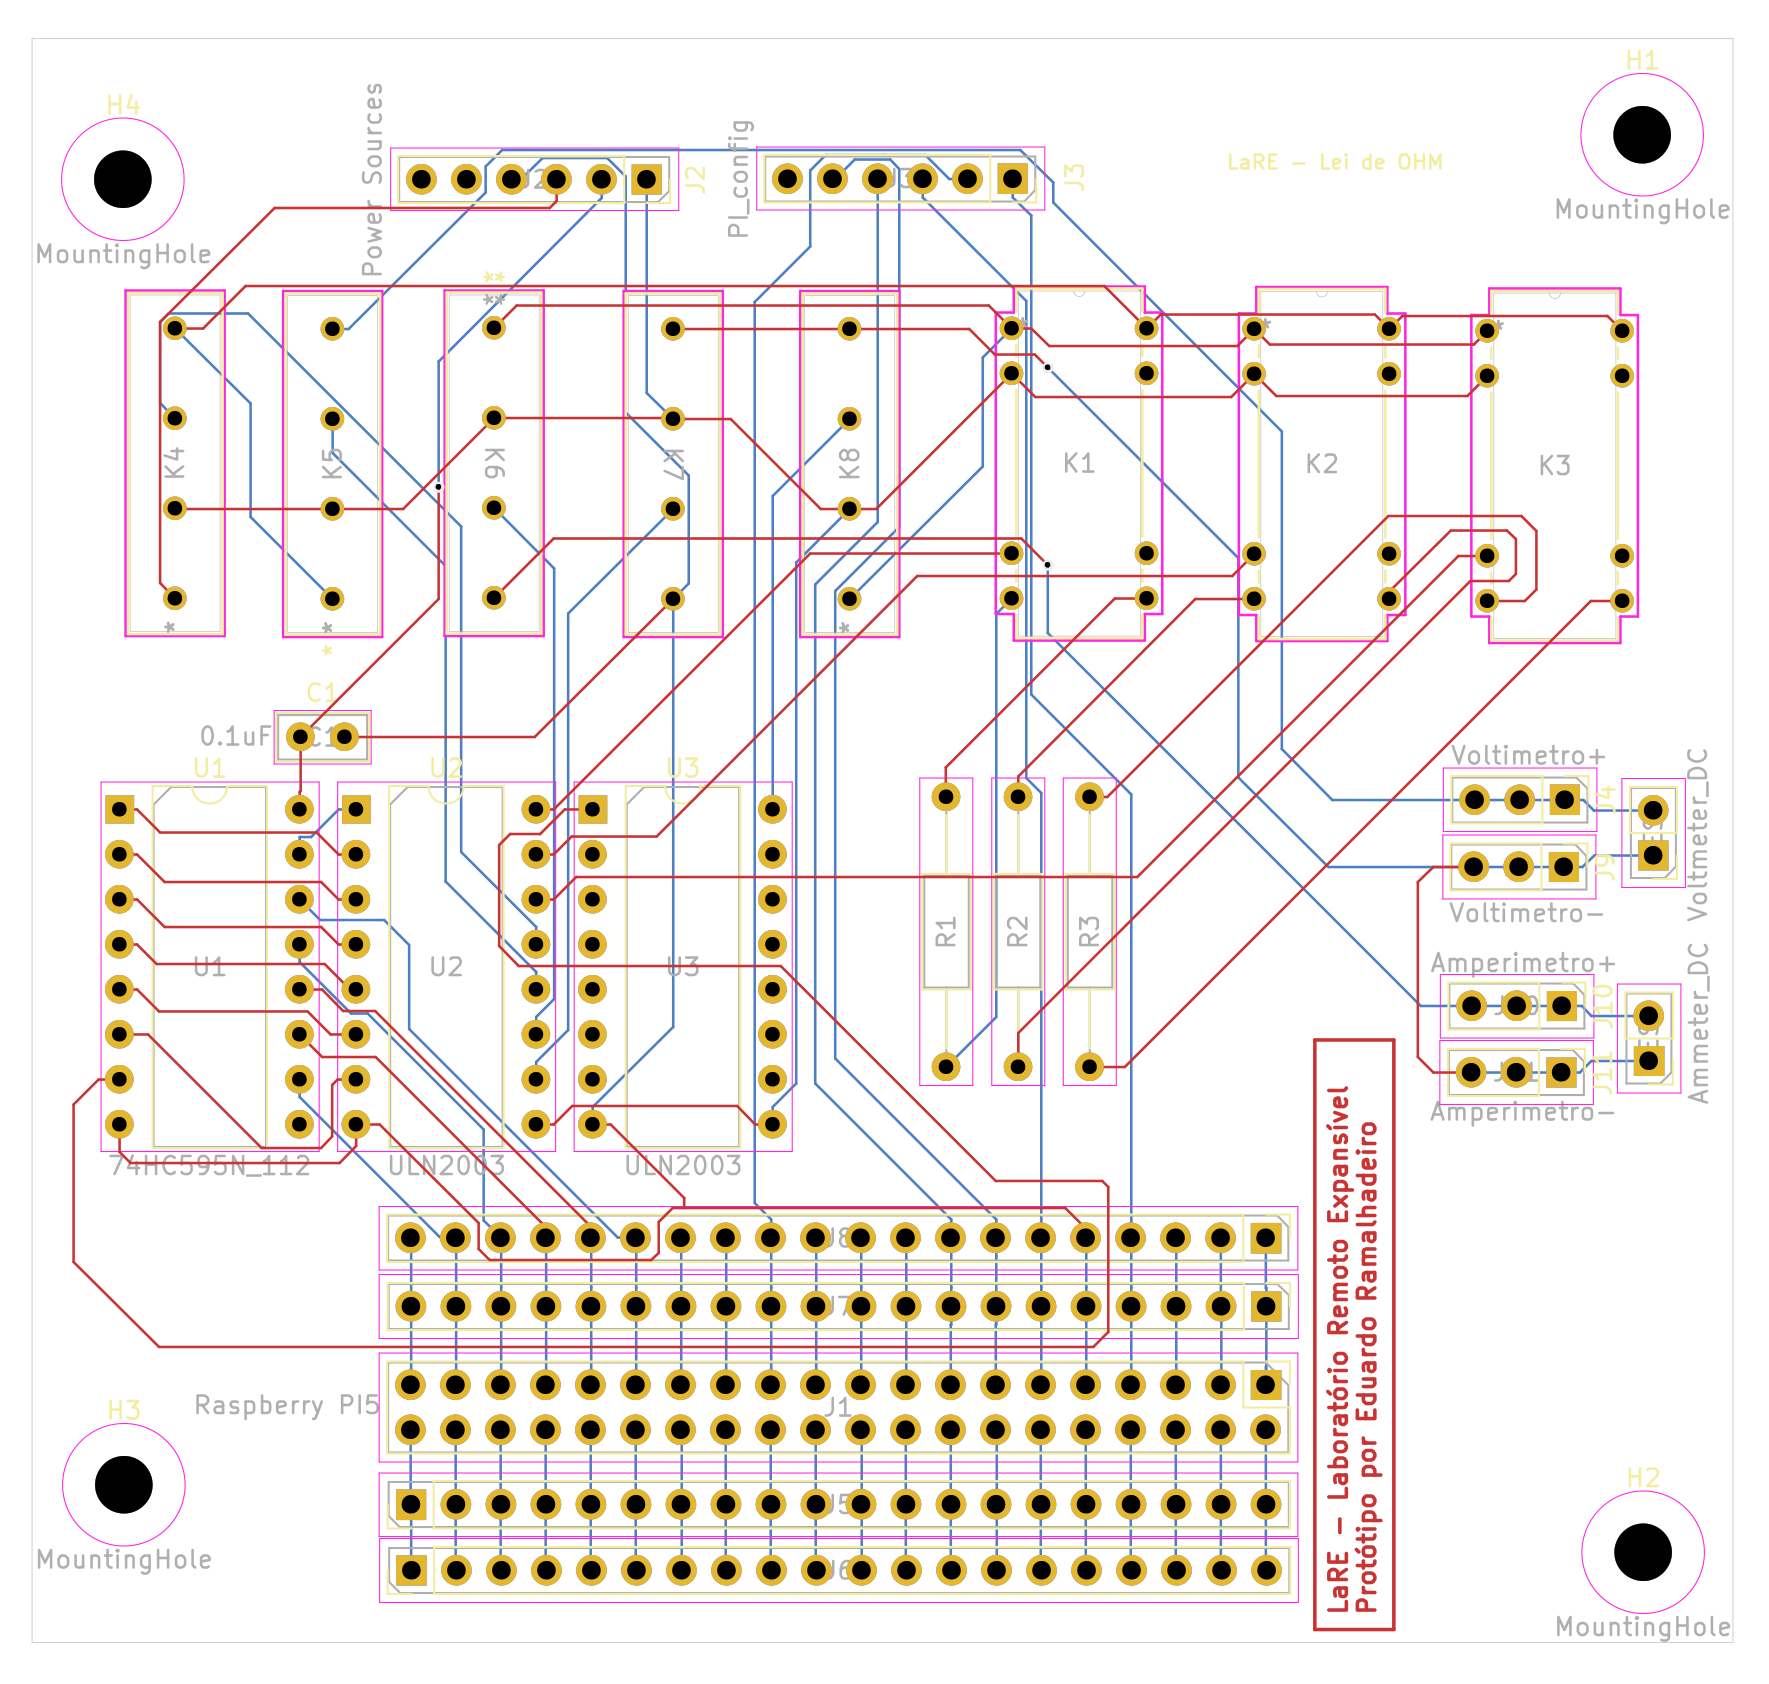
\includegraphics[width=1\textwidth]{figures/pcb_ohm.png}
    \caption{LaRE - PCB [Lei de Ohm]}
    \label{fig:pcbohm}
\end{figure}
\centering

\begin{figure}[hbtp]
    \centering
    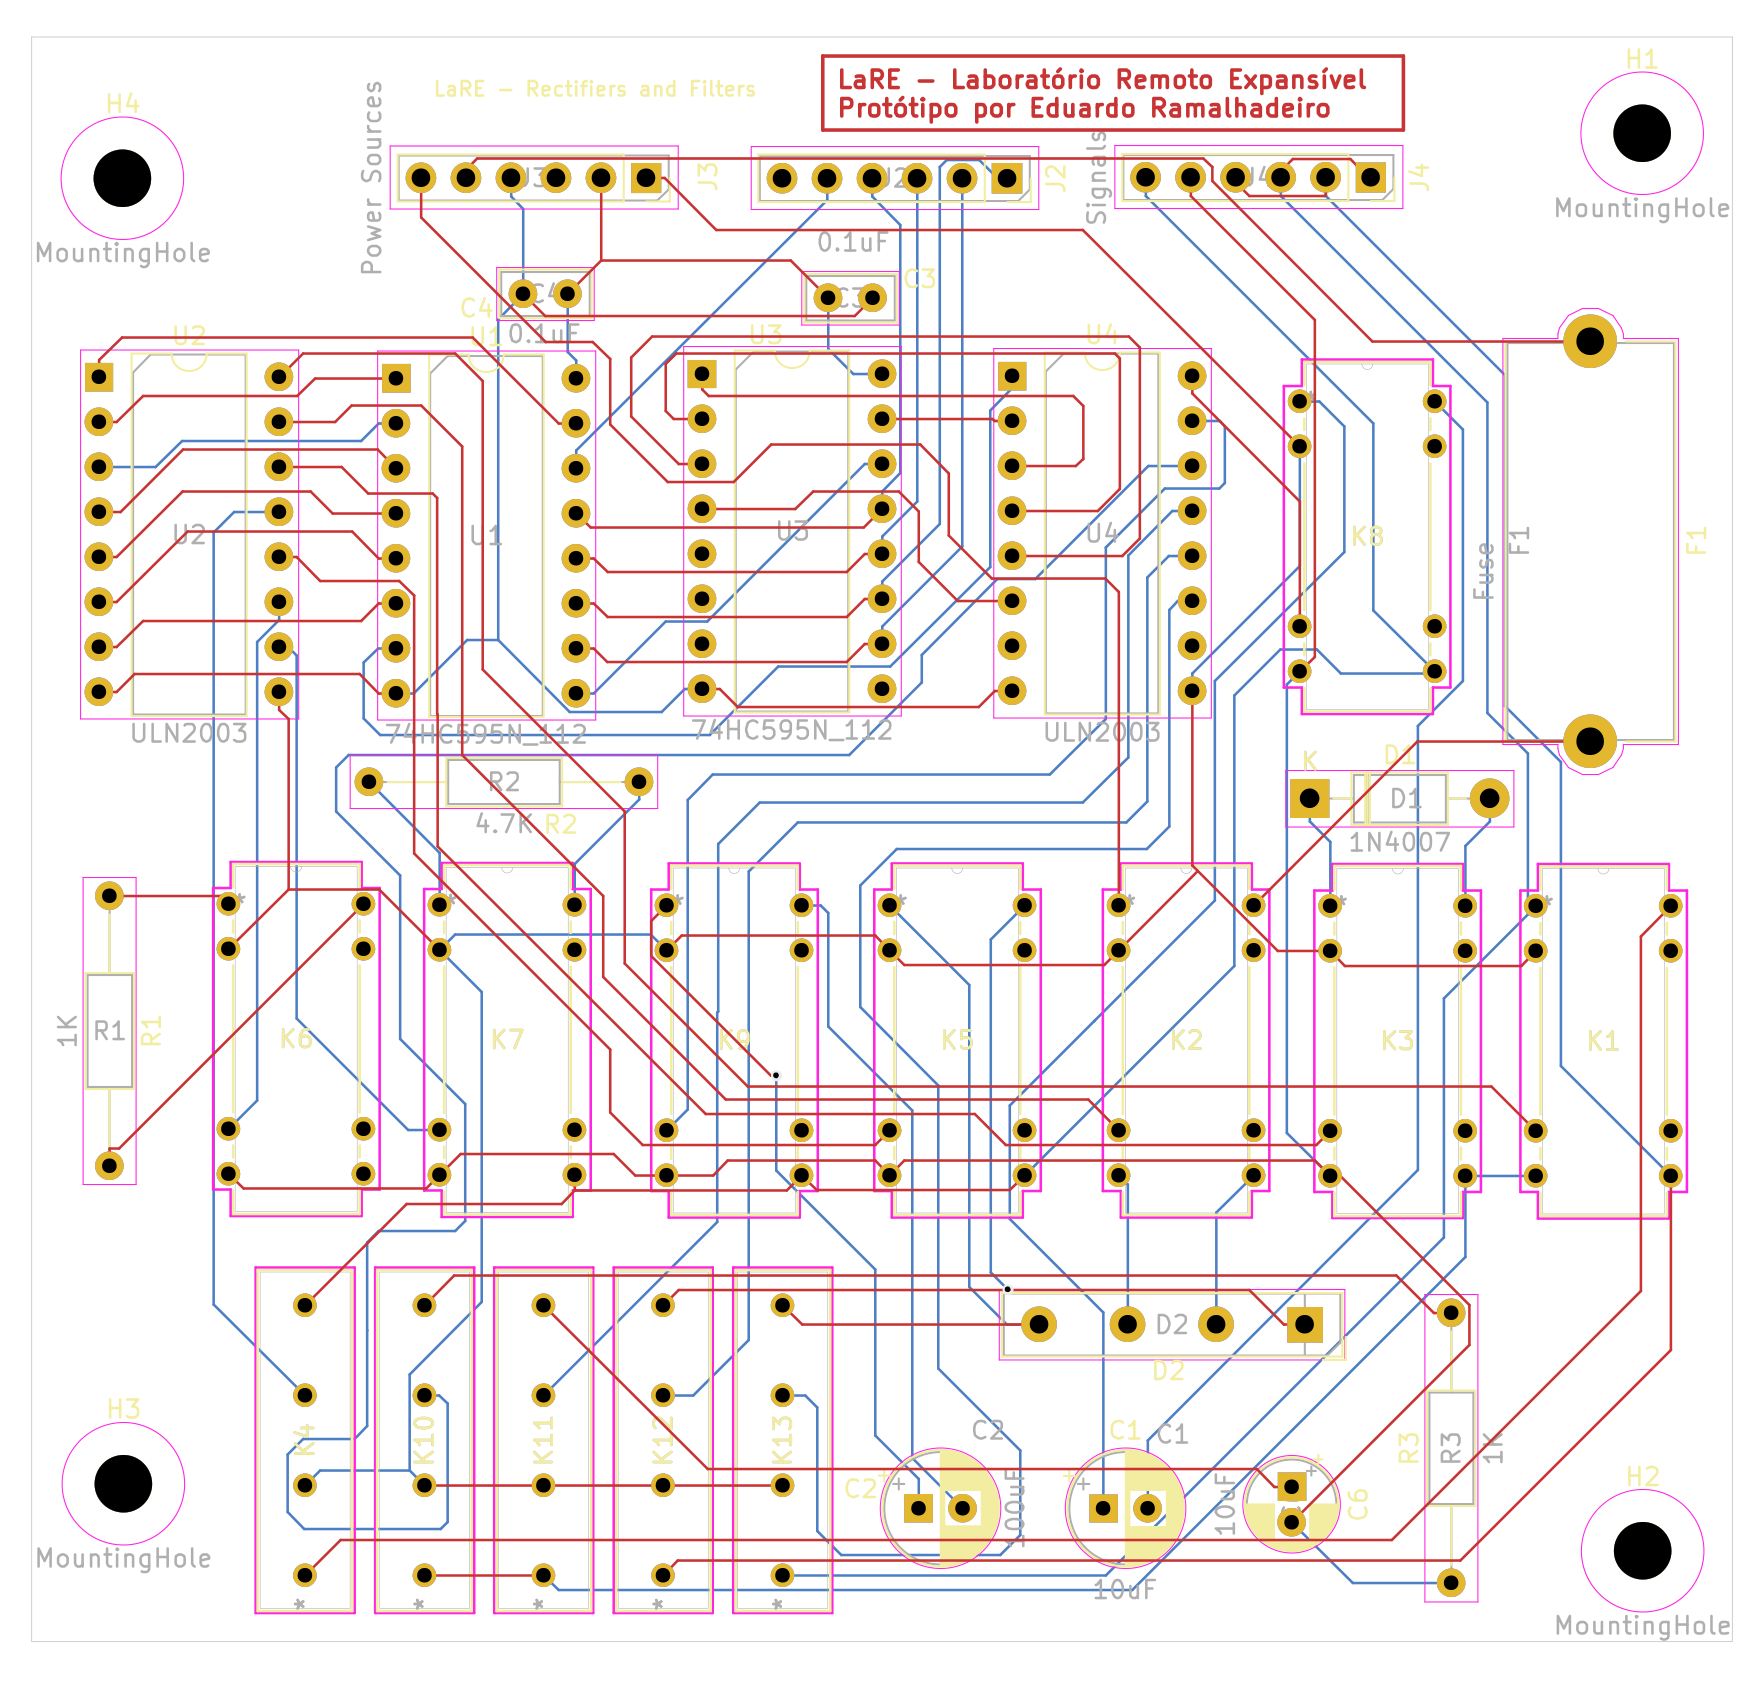
\includegraphics[width=1\textwidth]{figures/pcb_filtros.png}
    \caption{LaRE - PCB [Recficadores/Filtros]}
    \label{fig:pcbrectificador}
\end{figure}
\centering
